\PassOptionsToPackage{unicode=true}{hyperref} % options for packages loaded elsewhere
\PassOptionsToPackage{hyphens}{url}
%
\documentclass[]{article}
\usepackage{lmodern}
\usepackage{amssymb,amsmath}
\usepackage{ifxetex,ifluatex}
\usepackage{fixltx2e} % provides \textsubscript
\ifnum 0\ifxetex 1\fi\ifluatex 1\fi=0 % if pdftex
  \usepackage[T1]{fontenc}
  \usepackage[utf8]{inputenc}
  \usepackage{textcomp} % provides euro and other symbols
\else % if luatex or xelatex
  \usepackage{unicode-math}
  \defaultfontfeatures{Ligatures=TeX,Scale=MatchLowercase}
\fi
% use upquote if available, for straight quotes in verbatim environments
\IfFileExists{upquote.sty}{\usepackage{upquote}}{}
% use microtype if available
\IfFileExists{microtype.sty}{%
\usepackage[]{microtype}
\UseMicrotypeSet[protrusion]{basicmath} % disable protrusion for tt fonts
}{}
\IfFileExists{parskip.sty}{%
\usepackage{parskip}
}{% else
\setlength{\parindent}{0pt}
\setlength{\parskip}{6pt plus 2pt minus 1pt}
}
\usepackage{hyperref}
\hypersetup{
            pdftitle={Concurrent validity of an Estimator of Weekly Alcohol Consumption (EWAC) based on the Extended AUDIT},
            pdfborder={0 0 0},
            breaklinks=true}
\urlstyle{same}  % don't use monospace font for urls
\usepackage[margin=1in]{geometry}
\usepackage{longtable,booktabs}
% Fix footnotes in tables (requires footnote package)
\IfFileExists{footnote.sty}{\usepackage{footnote}\makesavenoteenv{longtable}}{}
\usepackage{graphicx,grffile}
\makeatletter
\def\maxwidth{\ifdim\Gin@nat@width>\linewidth\linewidth\else\Gin@nat@width\fi}
\def\maxheight{\ifdim\Gin@nat@height>\textheight\textheight\else\Gin@nat@height\fi}
\makeatother
% Scale images if necessary, so that they will not overflow the page
% margins by default, and it is still possible to overwrite the defaults
% using explicit options in \includegraphics[width, height, ...]{}
\setkeys{Gin}{width=\maxwidth,height=\maxheight,keepaspectratio}
\setlength{\emergencystretch}{3em}  % prevent overfull lines
\providecommand{\tightlist}{%
  \setlength{\itemsep}{0pt}\setlength{\parskip}{0pt}}
\setcounter{secnumdepth}{5}
% Redefines (sub)paragraphs to behave more like sections
\ifx\paragraph\undefined\else
\let\oldparagraph\paragraph
\renewcommand{\paragraph}[1]{\oldparagraph{#1}\mbox{}}
\fi
\ifx\subparagraph\undefined\else
\let\oldsubparagraph\subparagraph
\renewcommand{\subparagraph}[1]{\oldsubparagraph{#1}\mbox{}}
\fi

% set default figure placement to htbp
\makeatletter
\def\fps@figure{htbp}
\makeatother

\usepackage{booktabs}
\usepackage{longtable}
\usepackage{array}
\usepackage{multirow}
\usepackage{wrapfig}
\usepackage{float}
\usepackage{colortbl}
\usepackage{pdflscape}
\usepackage{tabu}
\usepackage{threeparttable}
\usepackage{threeparttablex}
\usepackage[normalem]{ulem}
\usepackage{makecell}
\usepackage{xcolor}
\usepackage[numbers]{natbib}
\bibliographystyle{vancouver}
\usepackage{dcolumn} 
\title{Concurrent validity of an Estimator of Weekly Alcohol Consumption (EWAC)
based on the Extended AUDIT}
\author{}
\date{\vspace{-2.5em}}

\begin{document}
\maketitle

{
\setcounter{tocdepth}{2}
\tableofcontents
}
\hypertarget{introduction}{%
\section{Introduction}\label{introduction}}

Globally, alcohol consumption is responsible for 5\% of all deaths and
disease burden \citep{Shield2020}. The burden of alcohol consumption
goes far beyond the burden of \emph{alcohol use disorders}, defined in
the International Statistical Classification of Diseases (ICD-10
F10.1/F10.2; ICD-11 QE10/6C40.1).

A number of strategies exist in order to either prevent
\citep{NICE-PH24}, or treat and reduce \citep{NICE-CG115} harm from
alcohol consumption. Some recommend systematic screening of alcohol use
disorders using a validated diagnostic tool. More recently, others have
advocated monitoring alcohol consumption like many other risk factors
(eg body mass index or cholesterol), making individuals more conscious
of their current intake and associated risk \citep{Nutt2014, Rehm2016}.
This approach is intended to enable timely lifestyle interventions (and,
if unsuccessful, pharmacological interventions), in order to prevent the
emergence of alcohol use disorders. Simultaneously, public health
recommendations to the public
\citep{AU.alcoguidelines2009, AlcoholCMO2016b} now promote the reduction
of alcohol consumption, in the absence of a `safe' level below which
alcohol does not increase disease risk \citep{Wood2018}.

In contrast with alcohol use disorder screening tools, alcohol
consumption assessment tools are not well embedded in clinical practice.
Potential reasons include: lack of diagnostic validation, difficulty to
self-assess alcohol consumption, and time pressures. This creates a gap
in the range of resources destined to help individuals understand,
monitor and take control of their alcohol consumption with--or
without--the involvement of primary care physicians.

The objective of this paper is to develop and validate a fast and
easy-to-complete Estimator of Weekly Alcohol Consumption (EWAC) by
repurposing an existing screening tool. In many countries, the most
widely used screening tool is the Alcohol Use Disorders Identification
Test (AUDIT) \citep{Babor2001}, a 10-item questionnaire schedule widely
employed in clinical practice and clinical research as a diagnostic test
for alcohol use disorder. The short, 3-item consumption version known as
AUDIT-C has good diagnostics accuracy for both: (a) interview-based
clinical diagnoses; and (b) consumption in excess of maximum recommended
intakes (eg 140g/week in Australia, 112 g/week in UK) in a variety of
populations \citep{DeMeneses-Gaya2009}.

The present study aims to validate the AUDIT-C against continuous
measures of alcohol consumption, as opposed to against a particular
clinical diagnosis or consumption threshold. To this end, we adopt a
variant of the AUDIT-C schedule known as the `Extended AUDIT-C', which
improves the granularity of the information collected with a greater
range of response options on quantity and frequency (AUDIT items 1 and
2). The Extended AUDIT-C has been used in UK research as part of two
trials \citep{Kaner2013c, Crane2018} and one continuous household survey
\citep{Beard2015a} to capture greater information on the higher risk
drinkers, based on the observation that AUDIT consumption items are
right-truncated.

This paper is made up of three investigations. Study 1 estimates
coefficients to apply to each of the AUDIT-C response items to compute
an EWAC using data from a large English household survey, the Alcohol
Toolkit Study (ATS). It then tests the concurrent validity of the EWAC
against Graduated-Frequency (GF) across a number of demographic
subpopulations in England. Study 2 tests the concurrent validity of the
EWAC against the 28-day Timeline Followback (TLFB) in a clinical
population (hospital clinic outpatients). Study 3 compares the
population-wide total and empirical cumulative distribution of alcohol
consumption in England using: the EWAC, the ATS graduated frequency
schedule, the Health Survey for England, and alcohol sales official
statistics.

\hypertarget{methods}{%
\section{Methods}\label{methods}}

\hypertarget{approach}{%
\subsection{Approach}\label{approach}}

This paper develops and validates an Estimator of usual Weekly Alcohol
Consumption in units (EWAC) based on the Extended AUDIT-C. Neither the
AUDIT-C nor the Extended AUDIT-C provide a measure of usual alcohol
consumption, but the product of frequency of drinking (AUDIT item 1) and
quantity of drinking (AUDIT item 2) can be used to estimate usual
alcohol consumption, with adjustment for occasional heavy use (AUDIT
item 3), following methods developed for quantity-frequency-variability
instruments \citep{Lemmens1992}.

In practice, for every individual \(i\), the EWAC is computed as the
product of \(F_i\) and \(Q_i\) (AUDIT items 1 and 2 respectively)
adjusted with the frequency of intense drinking \(V_i\) (AUDIT item 3):

\[\text{EWAC}_i = F_i Q_i + V_ib\]

where \(b\) denotes the average number of units of alcohol consumed in
an intense drinking day. Coefficients \(F, Q, V\) and \(b\) are unknown.
In this study, two sets of potential coefficients are evaluated:

\begin{itemize}
\tightlist
\item
  using the AUDIT response item interval midpoint: for example, 2.5 for
  `2 to 3 times per week' in AUDIT item 2
\item
  using a statistical model to estimate the coefficients directly from
  gold standard data.
\end{itemize}

All results are reported in UK alcohol units (8g or 10mL of pure
alcohol). Analyses are conducted in \texttt{R} \citep{RCoreTeam2017}
using packages \texttt{tidyverse} and \texttt{rstan}
\citep{package-tidyverse, package-rstan}. Computer scripts for all
analyses are available on an online repository \citep{Dutey2020}.

\hypertarget{data-sources}{%
\subsection{Data sources}\label{data-sources}}

A longstanding obstacle in alcohol research and care is the absence of a
diagnostic gold standard, which is not addressed even by the development
of new biomarkers. Instead, a number of instruments exist which measure
self-reported alcohol consumption with varying validity and reliability.
A state-of-the art review by \citep{Greenfield2000} is summarised in
Table 1 below. Prospective diaries tend to record higher alcohol
consumption by minimising recall bias, followed by GF, while lower
levels seem to be recorded with QF measures \citep{Heeb2005, Rehm1998}.

Table 1: Alcohol schedules: selective comparison

\begin{table}[H]
\centering
\begin{tabular}{l|l|l|l}
\hline
Schedule & Bias & Variance & Measures variability\\
\hline
Graduated frequency (GF) & Unclear & Low & Yes\\
\hline
Quantity-Frequency (QF) & Unclear & Low & No\\
\hline
Quantity-Frequency-Variability (QFV) & Unclear & Low & Yes\\
\hline
Yesterday' recall & Minimal & High & No\\
\hline
Timeline followback (TLFB) & Low & Low & Yes\\
\hline
Prospective diary & Low & Low & Yes\\
\hline
\end{tabular}
\end{table}

The present paper employs four sources of data presented in Table 2
below, together with references to methodological descriptions.

Table 2: Description of data sources

\begin{longtable}[]{@{}lllllrl@{}}
\toprule
\begin{minipage}[b]{0.12\columnwidth}\raggedright
Source\strut
\end{minipage} & \begin{minipage}[b]{0.12\columnwidth}\raggedright
Time\strut
\end{minipage} & \begin{minipage}[b]{0.12\columnwidth}\raggedright
Study population\strut
\end{minipage} & \begin{minipage}[b]{0.12\columnwidth}\raggedright
Measurements\strut
\end{minipage} & \begin{minipage}[b]{0.12\columnwidth}\raggedright
Validation\strut
\end{minipage} & \begin{minipage}[b]{0.07\columnwidth}\raggedleft
Sample size\strut
\end{minipage} & \begin{minipage}[b]{0.12\columnwidth}\raggedright
Design\strut
\end{minipage}\tabularnewline
\midrule
\endhead
\begin{minipage}[t]{0.12\columnwidth}\raggedright
Alcohol Toolkit Study (ATS) \citep{Beard2015a}\strut
\end{minipage} & \begin{minipage}[t]{0.12\columnwidth}\raggedright
November 2015--October 2017 (waves 110--133)\strut
\end{minipage} & \begin{minipage}[t]{0.12\columnwidth}\raggedright
Residents of private English households aged 16 years and over\strut
\end{minipage} & \begin{minipage}[t]{0.12\columnwidth}\raggedright
Interviewer-led Extended AUDIT-C and GF\strut
\end{minipage} & \begin{minipage}[t]{0.12\columnwidth}\raggedright
\citep{Heeb2005}, \citep{Greenfield2009}\strut
\end{minipage} & \begin{minipage}[t]{0.07\columnwidth}\raggedleft
40,832\strut
\end{minipage} & \begin{minipage}[t]{0.12\columnwidth}\raggedright
Cross-sectional sample survey\strut
\end{minipage}\tabularnewline
\begin{minipage}[t]{0.12\columnwidth}\raggedright
Health Survey for England (HSE) \citep{NatCenSocialResearch2013}\strut
\end{minipage} & \begin{minipage}[t]{0.12\columnwidth}\raggedright
2011\strut
\end{minipage} & \begin{minipage}[t]{0.12\columnwidth}\raggedright
Residents of private English households aged 16 years and over\strut
\end{minipage} & \begin{minipage}[t]{0.12\columnwidth}\raggedright
Interviewer-led beverage-specific QF\strut
\end{minipage} & \begin{minipage}[t]{0.12\columnwidth}\raggedright
Consistent with a prospective diary \citep{Boniface2014} and yesterday
recall \citep{Stockwell2016}.\strut
\end{minipage} & \begin{minipage}[t]{0.07\columnwidth}\raggedleft
8,610\strut
\end{minipage} & \begin{minipage}[t]{0.12\columnwidth}\raggedright
Cross-sectional sample survey\strut
\end{minipage}\tabularnewline
\begin{minipage}[t]{0.12\columnwidth}\raggedright
Hospital questionnaire study (HOSP)\strut
\end{minipage} & \begin{minipage}[t]{0.12\columnwidth}\raggedright
February 2019--October 2019\strut
\end{minipage} & \begin{minipage}[t]{0.12\columnwidth}\raggedright
Outpatient and day case hospital patients aged 18 years and over\strut
\end{minipage} & \begin{minipage}[t]{0.12\columnwidth}\raggedright
Interviewer/self-administered Extended AUDIT-C and interviewer-led
TLFB\strut
\end{minipage} & \begin{minipage}[t]{0.12\columnwidth}\raggedright
TLFB records fewer drinking days and thus lower consumption than a
prospective diary \citep{Grant1995}. This recall bias increases with the
number of days elapsed \citep{Hoeppner2010, Vinson2003}\strut
\end{minipage} & \begin{minipage}[t]{0.07\columnwidth}\raggedleft
130\strut
\end{minipage} & \begin{minipage}[t]{0.12\columnwidth}\raggedright
Cross-sectional study with block randomisation to (a) self-administered
AUDIT or (b) researcher-administered AUDIT.\strut
\end{minipage}\tabularnewline
\begin{minipage}[t]{0.12\columnwidth}\raggedright
Alcohol retail sales \citep{PHE2017}\strut
\end{minipage} & \begin{minipage}[t]{0.12\columnwidth}\raggedright
2014\strut
\end{minipage} & \begin{minipage}[t]{0.12\columnwidth}\raggedright
English population aged 18 years and over\strut
\end{minipage} & \begin{minipage}[t]{0.12\columnwidth}\raggedright
--\strut
\end{minipage} & \begin{minipage}[t]{0.12\columnwidth}\raggedright
\citep{PHE2017}\strut
\end{minipage} & \begin{minipage}[t]{0.07\columnwidth}\raggedleft
--\strut
\end{minipage} & \begin{minipage}[t]{0.12\columnwidth}\raggedright
Ratio of all alcohol produced or processed in the UK, as well as alcohol
imported into the UK for sale and consumption, over the mid-year
population estimate\strut
\end{minipage}\tabularnewline
\bottomrule
\end{longtable}

\hypertarget{study-1-ewac-estimation-and-concurrent-validity}{%
\subsection{Study 1: EWAC estimation and concurrent
validity}\label{study-1-ewac-estimation-and-concurrent-validity}}

Study 1 evaluates the accuracy of the EWAC derived from a
researcher-administered Extended AUDIT-C in community households. A
pre-registered protocol for this study is available online
\citep{Dutey2018}. It uses the GF schedule from the ATS as a gold
standard. Two sets of coefficients are compared: AUDIT response item
interval midpoint; and coefficients estimated using a statistical model
(supplementary material 1-2).

First, the agreement between the EWAC and the GF is quantified by
studying two types of deviations:

\begin{itemize}
\tightlist
\item
  bias is estimated using the mean deviation to the gold standard
  \(\text{MD} = n^{-1} \sum_{i=1}^{n}{(\rm{EWAC}_i - \rm{GF}_i )}\). We
  test the hypothesis that the MD is greater than 1 UK unit using a
  two-sided \(t\)-test.
\item
  precision is estimated using the root mean squared deviation
  \(\text{RMSD} = \sqrt{n^{-1} \sum_{i=1}^{n}{( \rm{EWAC}_i - \rm{GF}_i )^2}}\),
  a measure of total error: it capture both bias and random deviation
  from the assumed gold standard. For example, an RMSD of 2 signifies
  that the EWAC is on average with \(\pm\) 2 UK units of the gold
  standard. We test the hypothesis that the RMSD is greater than 2 UK
  units using a one-sided \(\chi^2\) homogeneity test.
\end{itemize}

Second, we examine whether the EWAC's validity varies across population
subgroups.

\begin{itemize}
\tightlist
\item
  the simple deviation \((\text{EWAC}-\text{GF})\) is regressed in a
  linear model to test for subgroup differences in MD
\item
  the squared deviation \((\rm{EWAC}-\rm{GF})^2\) is regressed in a
  log-transformed linear model to test subgroup differences in MSD.
  Model coefficients are then transformed (square root of the
  exponential) into relative RMSD estimates interpreted as the ratio of
  the subgroup RMSD to the reference category RMSD, a ratio
  \textgreater{}1 indicating worse precision than in the reference
  category.
\end{itemize}

Both models include the following predictors: sex by age group; ethnic
group; highest educational qualification; religion; smoking status.
Additional models are fitted solely in respondents with an AUDIT-C score
of 5 or more or an AUDIT score of 8 or more (under the ICD terminology,
hazardous and harmful alcohol use), using extra variables measures
during interview: favourite drink (beer; wine; spirits alone; mixed
spirits; cider; other); and whether the respondent attempt to restrict
alcohol intake in the last 12 months (eg by drinking less, choosing
lower strength alcohol or using smaller glasses).

Third, we test whether the EWAC is superior to the traditional AUDIT-C
score at predicting drinking in excess of 14 UK units per week. In the
UK, a score of 5 or more is categorised as `increasing risk' or `higher
risk', and regarded as indicating consumption in excess of 14 units per
week. The study tests the hypothesis that the EWAC's receiver operating
characteristics' area under the curve (AUC) is greater that the AUDIT-C
score using a nonparametric paired AUC test \citep{Delong1988}.

The ATS data (\(n=\) 40,832) is affected by missing data: 35\% of
respondents (\(n=\) 14,408) reported never drinking alcohol in AUDIT
item 1 and were not asked any further AUDIT or GF questions. These
participants are excluded from the analysis. A further 4,020 respondents
(0.2\% of those reporting drinking in AUDIT item 1) did not have a valid
GF alcohol consumption record and were also excluded. In total, 22,404
valid observations remain for the diagnostic analysis, in which missing
GF data is assumed to be missing at random conditionally on the Extended
AUDIT-C responses. In the subgroup analysis (Study 2 below), a further
530 repondents (0.5\%) were assumed to have data missing at random and
were excluded.

\hypertarget{study-2-concurrent-validity-in-hospital-outpatients}{%
\subsection{Study 2: Concurrent validity in hospital
outpatients}\label{study-2-concurrent-validity-in-hospital-outpatients}}

Study 2 aims to confirm the robustness of findings in (a) a clinical
population; (b) when the Extended AUDIT-C is self-administered; (c)
using a different gold standard: the 28-day TLFB. Participants were
recruited from a range of clinics at a large acute hospital in
Southampton, UK: orthopaedics, rheumatology, young adults, managed care
and mental health outpatients, as well as endoscopy day cases. A total
of 130 participants consented to participating, and block-randomised to
one of two groups:

\begin{enumerate}
\def\labelenumi{(\arabic{enumi})}
\tightlist
\item
  self-administered Extended AUDIT-C (n=59)
\item
  researcher-administered Extended AUDIT-C (n=71).
\end{enumerate}

Once this first questionnaire completed, both groups were asked to
complete a 28-day alcohol TFLB questionnaire administered by the
researcher.

To model the relationship between the EWAC and the TLFB, the number of
units consumed on any day is assumed to follow a negative binomial
distribution, the rate of which is determined by the latent usual
alcohol consumption as well as the following variables: AUDIT mode of
administration (self-administered; researcher-administered), week day,
number of days elapsed since (1-7; 8-14; 15-21; 22-28). TLFB daily
number of units consumed were rounded to the nearest integer and
regressed in a negative binomial regression model against the
aforementioned predictors, as well as the EWAC divided by 7 to obtain
its daily equivalent. The corresponding regression coefficient measures
the ratio of TLFB to EWAC.

\hypertarget{study-3-aggregate-concurrent-validity}{%
\subsection{Study 3: Aggregate concurrent
validity}\label{study-3-aggregate-concurrent-validity}}

Study 3 examines the consistency in aggregate alcohol consumption
estimates across England in residents aged 18 years and over. We plot
plot the empirical cumulative distributions of alcohol consumption given
by (1) the EWAC estimated from the ATS; (2) the quantity-frequency
estimated in the ATS; (3) the beverage-specific estimators in HSE in
2011; (4) the prospective diary estimator in HSE 2011. In this analysis,
survey weights are used: in (1-3), poststratification weights estimated
using calibration and age-sex MYPES; in (4), similar postratification
weights adjusted for self-selection into participation to the
prospective diary data collection. We report the percentage of total
alcohol sales for England accounted for by each method, using both
on-trade and off-trade 2014 sales estimates for England from
\citep{PHE2017}.

\hypertarget{results}{%
\section{Results}\label{results}}

\hypertarget{study-1-ewac-estimation-and-validation}{%
\subsection{Study 1: EWAC estimation and
validation}\label{study-1-ewac-estimation-and-validation}}

\hypertarget{overall-bias-and-accuracy}{%
\subsubsection{Overall bias and
accuracy}\label{overall-bias-and-accuracy}}

The first step involved choosing a set of coefficients to compute the
EWAC (supplementary materials 1--2).

The EWAC computed with the midpoint of the AUDIT item intervals has a
Pearson's correlation \(r\) = 0.69, {[}95\% CI: 0.69, 0.70{]}. It
produces a mean deviation (MD) of 0.71 UK alcohol units/week, indicating
a bias inferior to the preregistered \(\pm\) 1-unit bias allowance
(\(p\) = 1.000). The root mean squared deviation (RMSD) estimate of 12.3
units {[}95\% CI: 11.2;13.2{]} is significantly greater than the
pre-registered 2-unit total error allowance (\(p\) \textless{} 0.001),
suggesting that the EWAC falls on average 12 units away from the GF gold
standard.

Coefficients estimated empirically (statistical model reported in
supplementary materials 2) provide a small improvement: \(r\) = 0.71
{[}0.71, 0.72{]} (Kendall's rank correlation \(\tau\) = .63) and MD =
0.18 (\(p\) = 1.000). With RMSD = 10.9 {[}95\% CI: 9.8;12.0{]},
precision remains statistically significantly greater than 2 (\(p\)
\textless{} 0.001).

The RMSD masks a dispersed and skewed distribution of error. Table 3
shows that, for 50\% of participants, the EWAC falls within \(\pm\) 2 UK
units of the GF weekly consumption estimate. In other terms, an interval
estimate defined as the EWAC \(\pm\) 2 units (eg `10 to 14 units') would
cover the gold standard for half of individuals, while an interval
estimate defined as the EWAC \(\pm\) 3 units (eg `9 to 15 units') would
cover the gold standard for 60\% of individuals.

Table 3: Percentiles of the absolute deviation between EWAC and GF
schedule (n = 22,404)

\begin{tabular}{l|l|l|l|l|l|l|l|l|l|l}
\hline
10\% & 20\% & 30\% & 40\% & 50\% & 60\% & 70\% & 80\% & 90\% & 95\% & 99\%\\
\hline
0.4 & 0.7 & 1.0 & 1.5 & 2.1 & 3.0 & 4.2 & 6.2 & 10.6 & 17.0 & 38.7\\
\hline
\end{tabular}

Figure 1 compares individual EWAC and GF values. We note the departure
of lines of best fit from the diagonal, demonstrating the EWAC's small
positive bias (MD \textgreater{} 0) is not consistent. The plots
indicate a slight positive bias for consumptions up to 10-14 units/week,
then a slight negative bias above this threshold.

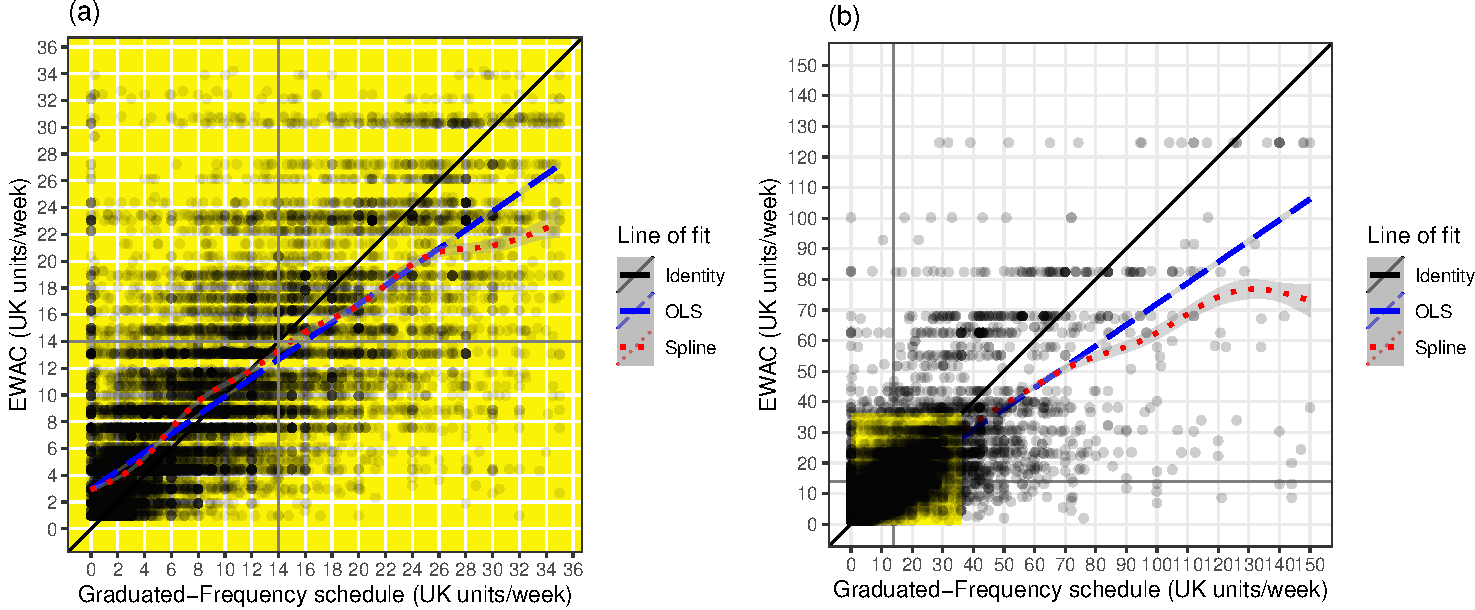
\includegraphics{analysis_files/figure-latex/unnamed-chunk-2-1.pdf}

Figure 1: Plots of EWAC against GF in (a) low/increasing risk ATS
respondents (n=21,338) and (b) all ATS respondents (n=22,373)

\hypertarget{subgroup-accuracy}{%
\subsubsection{Subgroup accuracy}\label{subgroup-accuracy}}

Next, the MD and RMSD are regressed against respondent characteristics
in order to identify subgroups with heterogeneous bias or precision
(supplementary material 3, Table 7). The reference category's key
characteristics are: females aged between 25 and 34 years of White
ethnicity without educational qualifications, who never smoked. The
model predictors explain a very modest proportion of both MD and RMSD
(\(R^2\) statistics \textless{} 2\%). Nevertheless, specific subgroups
do exhibit very different MD and RMSD.

Figure 7 summarises the MD for a selection of subgroups whose predicted
MD was either above 1 or below -1; and whose coefficients had a
\(p\)-value below 0.05. Respondents of Black, Other, and White Other
ethnic groups had significantly overestimated EWACs: their MDs were
respectively 4.8 units {[}95\% CI: 2.1, 7.5{]}; 5.9 units {[}1.6,
10.1{]} and 1.6 {[}0.2, 3.0{]} in excess of the reference MD. The MDs of
respondents aged 55 to 64 years or 75 years and over respectively had
MDs 2.2 units {[}0.5; 3.9{]} and 4.2 units {[}0.9; 7.6{]} in excess of
the reference MD. Similar results were found in increasing risk
drinkers, without significant evidence of an effect of favourite drink
or attempts to reduce alcohol intake in the past year (supplementary
material 3, Table 8)

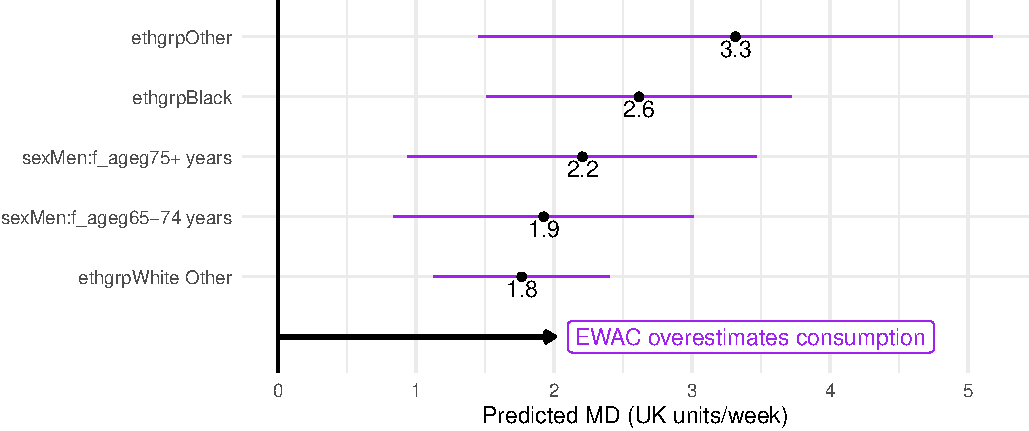
\includegraphics{analysis_files/figure-latex/ewac_subgroup_bias-1.pdf}

Figure 2: Forest plot of modelled MD for selected subgroups

Figure 3 shows those subgroups with an RMSD found to be significantly
different from the rest of the population (\(p < 0.05\)); and estimated
to be 20\% greater or smaller than the RMSD of the reference category.
This shows that RMSD is 58\% {[}95\% CI: 50; 67\%{]} greater in current
smokers, 34\% {[}14; 56\%{]} greater in respondents who stopped smoking
in the past year, and 23\% greater {[}17; 30\%{]} in respondents who
stopped smoking over a year ago. It is also 44\% greater {[}29; 60\%{]}
greater in men and 34\% greater {[}19; 50\%{]} in respondents aged 16 to
24 years. Conversely, error is 35 to 70\% smaller in White Other, Black
and Other ethnic groups.

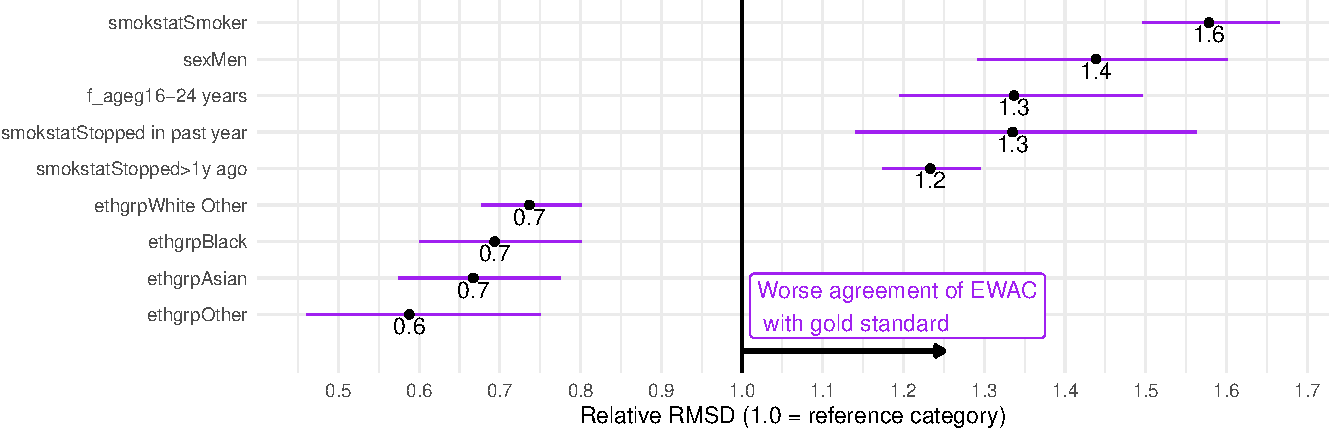
\includegraphics{analysis_files/figure-latex/ewac_subgroup_error-1.pdf}

Figure 3: Forest plot of RMSD ratio (selected subgroups to reference
category)

Figure 4 visualises the same analysis in increasing risk drinkers
exclusively (AUDIT-C \(\geq\) 5 or AUDIT \(\geq\) 8). With a higher mean
alcohol consumption, results differ from the overall picture presented
in Figure 3. The RMSD of respondents favouring mixed spirits had an RMSD
23\% {[}95\% CI: 9.6; 38{]} smaller than the reference category.
Educational qualifications seem to significantly improve the agreement
between EWAC and the gold standard. School and degree-level
qualifications reduced RMSD by 24\% {[}12; 37\%{]} and 37\% {[}23;
52\%{]} smaller respectively with unchanged MD, suggesting that
respondents may have better recall and clarity over alcohol beverage
content. Conversely, the RMSD of respondents who attempted to reduce
their alcohol consumption was 23\% {[}16; 30\%{]} larger than the
reference category.

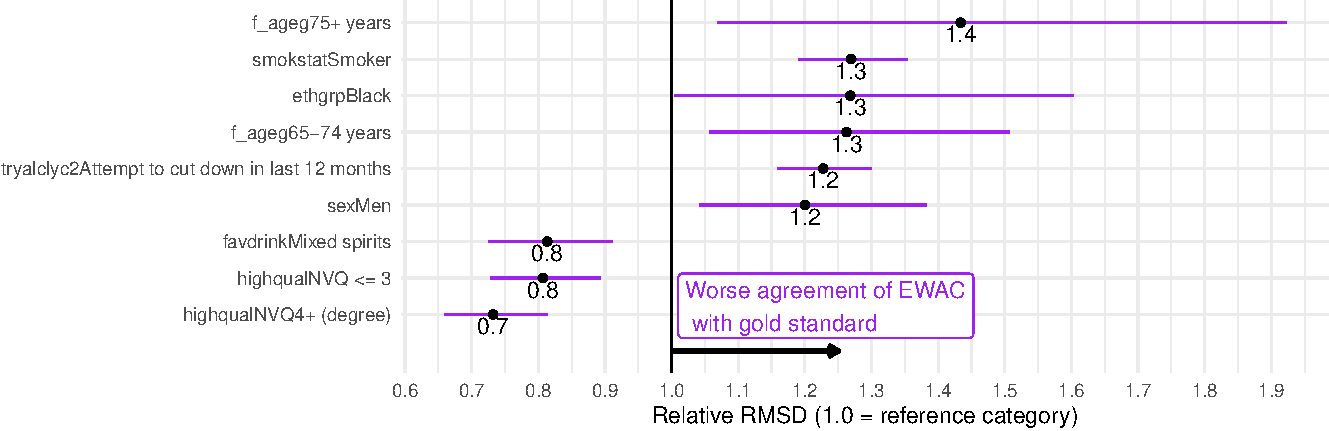
\includegraphics{analysis_files/figure-latex/ewac_subgroup_error_increasedrisk-1.pdf}

Figure 4: Forest plot of RMSD ratio (selected subgroups to reference
category) in respondents with a hazardous/harmful alcohol use
(AUDIT-C\textgreater{}=5 or AUDIT\textgreater{}=8

\hypertarget{receiver-operating-characteristics}{%
\subsubsection{Receiver Operating
Characteristics}\label{receiver-operating-characteristics}}

The last step of this analysis was to examine the EWAC's ability to
classify participants' consumption as being equal or in excess of 14 UK
units/week. In comparison with the AUDIT-C score (ranging 0-12), EWAC
increases the area under the curve by 5 percentage points (Table 4), a
statistically significant improvement (\(p\) \textless{} 0.001). ROC
curve are available from Supplementary Material 3. The cut-off that
maximises the sum of specificity and sensitivity is 9.95 units/week. In
constrast, using the nominal cut-off of 14 units/week yields a
sensitivity of 0.705 and a specificity of 0.922.

In summary, using an EWAC threshold of 10 units or more over an AUDIT-C
score of 5 or more provides equivalent sensitivity, but with an a steep
gain in specificity of 13 percentage points.

Table 4: Receiver operating characteristics of AUDIT-C score and EWAC
for consumption \textgreater{}= 14 UK units/week (n = 22,404)

\begin{tabular}{l|r|l|r|r|r}
\hline
Metric & AUC & 95\% CI & Best threshold & Sensitivity & Specificity\\
\hline
AUDIT-C score & 0.871 & [0.866; 0.876] & 4.50 & 0.882 & 0.684\\
\hline
EWAC & 0.921 & [0.917; 0.925] & 9.95 & 0.876 & 0.816\\
\hline
\end{tabular}

\emph{Note}: The best threshold refers the cut-off value that maximises
the sum of sensitivity and specificity.

\hypertarget{study-2-concurrent-validity-in-hospital-patients}{%
\subsection{Study 2: Concurrent validity in hospital
patients}\label{study-2-concurrent-validity-in-hospital-patients}}

A total of 105 participants (81\%) completed the Extended AUDIT-C, of
whom 63 were classified as low-risk drinkers, 25 as increasing-risk
alcohol users (AUDIT-C score of 5 to 7), and 17 as high-risk alcohol
users (AUDIT-C score of 8 or more). A total of 13 participants did not
provide TLFB information for at least one day missing out of 28,
resulting in 5\% (137/2940) of TLFB days were missing.

Using only 103 participants with a minimum of 7 days recorded on the
TLFB, MD is estimated at -0.5 unit/week, which does not provide any
evidence of bias greater than 1 unit/week (\(p\) = 0.316). As for error,
RMSD is estimated at 5.4 {[}95\%CI: 3.5; 6.8{]} and is statistically
significantly greater than 2 units (\(p\) \textless{} 0.001). A
potential reason for RMSD being considerably smaller than in Study 1 is
the distribution of alcohol consumption of this small pilot dataset.
Respondents' alcohol intake as estimated by TLFB was low, with a mean of
7 units/week; a median of 2 units/week, and a 90th percentile of 23
units/week. Consequently, the probability of observing the strong
deviations that can be observed in presence of high alcohol consumption
data was low.

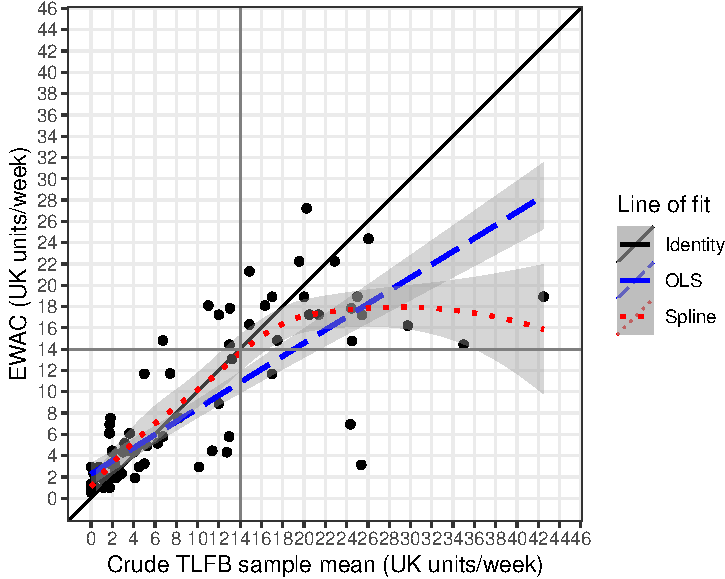
\includegraphics{analysis_files/figure-latex/tlfb_scatterplot-1.pdf}

Figure 5: Plot of EWAC estimates against TLFB estimates in hospital
participants with lines of fit

\hypertarget{study-3-empirical-distribution-functions}{%
\subsection{Study 3: Empirical distribution
functions}\label{study-3-empirical-distribution-functions}}

Table 6 provides estimates of total alcohol consumption in adult
resident of private households in England using four different
estimators, and compares them with alcohol retail sales. The HSE
schedules provide the highest estimates of alcohol consumption and
coverage of sale statistics. The proposed EWAC estimates of total
consumption are just 71\% of a very reliable estimate, the HSE
prospective diary.

Table 6: Summary statistics on alcohol consumption in England in
residents aged 18 years and over (excluding abstainers)

\begin{longtable}[]{@{}lrrrrr@{}}
\toprule
Study & Mean (units/week) & Median & Variance & N & \% of alcohol
sold\tabularnewline
\midrule
\endhead
HSE beverage-specific QF & 14.0 & 7.3 & 474.6 & 6,545 &
72.6\tabularnewline
HSE prospective diary & 13.0 & 8.0 & 264.7 & 4,640 & 67.6\tabularnewline
ATS GF & 8.5 & 5.1 & 242.0 & 22,136 & 44.0\tabularnewline
ATS EWAC & 9.3 & 5.2 & 148.9 & 25,882 & 48.0\tabularnewline
Retail sales & 19.3 & -- & -- & -- & --\tabularnewline
\bottomrule
\end{longtable}

Figure 6 suggests that the EWAC, like the ATS GF it was estimated
against, estimates a higher prevalence of low risk consumption (\(\leq\)
14 units/week) and increased risk consumption than HSE. In contrast very
high alcohol consumption (\(\geq\) 50 units/week) is higher in HSE. This
may be due to a combination of difference in sampling coverage,
nonresponse bias, or measurement error in the alcohol schedules.

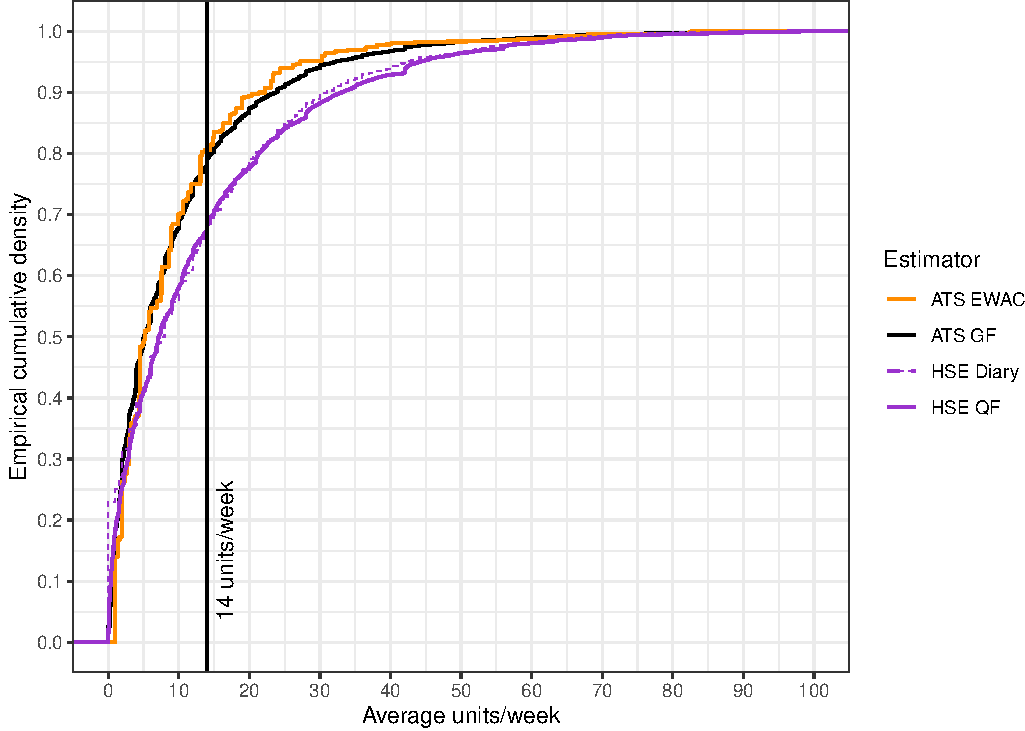
\includegraphics{analysis_files/figure-latex/ggplot_ECDF-1.pdf}

Figure 6: Empirical cumulative distribution function of weekly alcohol
consumption in England according to four alcohol schedules in residents
aged 18 years and over

\hypertarget{discussion}{%
\section{Discussion}\label{discussion}}

\hypertarget{main-findings}{%
\subsection{Main findings}\label{main-findings}}

This paper examined the predictive capabilities of the Extended AUDIT in
assessing alcohol consumption in two English populations: community
dwelling household residents, and hospital clinic outpatients. The
Extended AUDIT is a variant of the AUDIT-C containing a choice of 6
response items to quantify drinking frequency, and 7 reponse items to
quantify the average quantity consumed during any drinking day. The
resulting EWAC estimates usual alcohol consumption with a mean precision
of \(\pm\) 11 units/week when compared to the GF alcohol schedule, or
\(\pm\) 5 units/week when compared to a 28-day TLFB in a sample of
lower-risk alcohol users. Although bias is mostly consistent across
subgroups examined (age/sex, education, smoking status, religion), there
is strong evidence that EWAC overestimates alcohol consumption by 2-3
units/week in Black and Other ethnic groups. At the same time, average
precision is better in Black, Asian and Other ethnic groups. This is
likely due to a lower mean alcohol consumption than White British and
Mixed ethnic groups. We also noted a weaker precision for both current
and ex-smokers.

\hypertarget{strengths-and-limitations}{%
\subsection{Strengths and limitations}\label{strengths-and-limitations}}

To the best of our knowledge, this study was the first to (a) develop an
EWAC using a well-accepted clinical alcohol use disorders identification
tool such as the AUDIT; and (b) quantify its bias and precision with
respect to a continuous measure of alcohol consumption. One study by
\citep{Rubinsky2013} previously reported mean consumption by AUDIT-C
score, yet without quantifying bias or precision of such a measure.
Other studies have studied the AUDIT-C's potential in estimating alcohol
consumption, but only in relation to predicting consumption in excess of
a predefined threshold \citep{DeMeneses-Gaya2009}. Such studies achieved
AUCs ranging .83-.96. Study 1 demonstrated the EWAC's superiority for
predicting GF \(\geq\) 14 units/week. While its AUC of 0.921 {[}95\% CI:
0.917; 0.925{]} is comparable with many other studies, the specificity
gain from .684 to .876 places the EWAC in line with the best-performing
validations.

This study should provide strong confidence in the internal and external
validity of findings in England on account of the large sample size of
the ATS, the range of subgroup analyses reported, and replication of the
analysis in a clinical population using the TLFB method (Study 2).

We note some limitations. Findings reported in this paper may not apply
to other countries, or to small subpopulations in England with an
atypical alcohol consumption, such as patients seeking care for
conditions such as addition or alcohol liver disease. Alcohol survey
data quality issues also raise questions of internal validity in Study
1.

The gold standard has a strong influence on estimates of precision
(RMSD). Error in the gold standard will entirely propagate to the RMSD
measure (unless this error correlates with error in the EWAC). This
means some of the RMSD may in fact be due to error in the gold standard
rather than the EWAC. In a telephone interview study on 119 participants
in San Fransisco, US, \citep{Greenfield2009} measured a Pearson's
correlation coefficient of \(r\) = .86 and .87 in drinking frequencies
and volumes measured by a GF interview followed by a 28 day prospective
diary. In a telephone interview study of 773 participants across
Switzerland, \citep{Heeb2005} measure a Kendall's rank correlation
\(\tau\) = 0.41 between GF and a 7-day prospective diary. For reference,
our study measured a correlation coefficient \(r\) = .71 and \(\tau\) =
.63 between EWAC and GF. Our measures of RMSD are thus likely to be very
conservative estimators of precision.

The ATS, in spite of a large sample size, may suffer from coverage
issues. Like the HSE, ATS does not cover populations excluded from most
sampling frames, such as residents of communal and carceral
institutions, homeless people, or migrant populations. Independently
from coverage, evidence suggests that survey nonrespondents may have
higher alcohol consumption and harm, suggesting they may concentrate
high levels of alcohol consumptions
\citep{Gorman2014, Christensen2015, Boniface2017}. Furthermore, ATS
potentially misses some (mostly low-risk) drinkers, even among
respondents. \citep{DeVocht2016} noted that the proportion of
respondents classified as non-drinkers (based on AUDIT item 1) in ATS is
10\% higher than in HSE, in which respondents are asked to confirm
whether they never drink alcohol, or only drink `very occasionally'. All
these factors are likely to explain some of the discrepancy visible in
Study 3, but also affect MD and RMSD estimates reported in Study 1.

\hypertarget{potential-applications}{%
\subsection{Potential applications}\label{potential-applications}}

While retaining the AUDIT's strengths (speed, accuracy, international
standardisation), the Extended AUDIT improves the granularity of the
information collected on alcohol consumption, and captures greater
information from higher-risk drinkers, by remediating the
right-truncation of the traditional AUDIT consumption items. The EWAC
enhances the Extended AUDIT's health education and promotion qualities,
by translating it into an understandable scale: alcohol consumption.
This has the merit of focusing the recipient's attention to alcohol
units or grams, and can facilitate uptake with brief interventions
targetting skills in recognising the alcohol content of different drinks
and drink sizes to reduce consumption.

This may be particularly relevant as part of efforts to provide earlier
interventions (identification and brief advice) to increasing-risk
drinkers, to prevent (instead of treat) alcohol use disorders
{[}\citep{Lavoie2010};{]}. Knowledge of alcohol beverage content is not
universal. Many countries have not adopted a measure of standard drinks
\citep{Kalinowski2016}. In England, two thirds of drinkers could assess
the standard drink equivalent in wine or beer of one alcohol unit
\citep{ONS2009}.

Contributions by \citep{Nutt2014} and \citep{Rehm2016} are an incentive
to adopt a more clinical approach to alcohol use disorders prevention,
treating alcohol consumption like any other risk factor: blood pressure
or cholesterol are frequently monitored by general physicians in a non
stigmatising way and can act as a trigger for health intervention. In a
similar way, \citep{Nutt2014} and \citep{Rehm2016} argue that alcohol
use disorders are best prevented if individuals know their consumption,
and general practitioners can engage with patients effectively in
managing risks, first with lifestyle interventions and, if relevant,
pharmacological alternatives.

The proposed EWAC can fulfil the same alcohol use disorder screening
functions as the AUDIT-C, while at the same time providing transparent
information to patients in a less stigmatising way than terminology
previously in use (hazardous and harmful drinking). Communication of an
alcohol consumption estimate can motivate increasing risk drinkers to
monitor their consumption, while at the same time encouraging low-risk
drinkers to maintain this lifestyle. Its format is particularly suitable
for digital intervention. Study 3 suggests that the EWAC is as reliable
when the Extended AUDIT-C is self-administered as when it is
administered by a researcher. The EWAC can be part of personalised
feedback in a digital brief intervention, based on the overall
consumption estimate as well as the intensity of alcohol consumption
(AUDIT item 3).

\hypertarget{ethics}{%
\section{Ethics}\label{ethics}}

Study 1 and 3 were approved by the University of Southampton's Faculty
of Medicine Ethics Committee (ERGO 44682). Study 2 was approved by the
Health Research Authority National Research Ethics Service (IRAS 247458;
REC 18/SC/0564).

\hypertarget{supplementary-materials}{%
\section{Supplementary materials}\label{supplementary-materials}}

\hypertarget{supplementary-materials-1-ewac-coefficients-csv-file}{%
\subsection{Supplementary materials 1: EWAC coefficients (CSV
file)}\label{supplementary-materials-1-ewac-coefficients-csv-file}}

\hypertarget{supplementary-materials-2-bayesian-model-report-pdf-file}{%
\subsection{Supplementary materials 2: Bayesian model report (PDF
file)}\label{supplementary-materials-2-bayesian-model-report-pdf-file}}

\hypertarget{supplementary-materials-3-subgroup-analyses}{%
\subsection{Supplementary materials 3: Subgroup
analyses}\label{supplementary-materials-3-subgroup-analyses}}

Table 7: Coefficients of linear regression of the bias and error of EWAC
compared with GF in all respondents (n = 21,874)

\% Table created by stargazer v.5.2.2 by Marek Hlavac, Harvard
University. E-mail: hlavac at fas.harvard.edu \% Date and time: Sun, Feb
16, 2020 - 23:16:30 \% Requires LaTeX packages: dcolumn

\begin{table}[!htbp] \centering 
  \caption{} 
  \label{} 
\begin{tabular}{@{\extracolsep{5pt}}lD{.}{.}{-1} D{.}{.}{-1} } 
\\[-1.8ex]\hline 
\hline \\[-1.8ex] 
\\[-1.8ex] & \multicolumn{1}{c}{(EWAC\_QFV - GFMEANWEEKLY)} & \multicolumn{1}{c}{LOG((EWAC\_QFV - GFMEANWEEKLY)$^2$)} \\ 
\\[-1.8ex] & \multicolumn{1}{c}{1} & \multicolumn{1}{c}{2}\\ 
\hline \\[-1.8ex] 
 Constant & 0.7$ $(-0.1$, $1.5) & 0.7$ $(0.5$, $0.9)^{***} \\ 
  sexMen & -1.2$ $(-2.0$, $-0.4)^{**} & 0.7$ $(0.5$, $0.9)^{***} \\ 
  f\_ageg16-24 years & 0.7$ $(-0.1$, $1.6) & 0.6$ $(0.4$, $0.8)^{***} \\ 
  f\_ageg35-44 years & -0.6$ $(-1.4$, $0.2) & 0.03$ $(-0.2$, $0.2) \\ 
  f\_ageg45-54 years & 0.03$ $(-0.7$, $0.8) & 0.1$ $(-0.1$, $0.3) \\ 
  f\_ageg55-64 years & 0.5$ $(-0.3$, $1.3) & 0.1$ $(-0.1$, $0.3) \\ 
  f\_ageg65-74 years & 0.1$ $(-0.8$, $0.9) & -0.2$ $(-0.4$, $0.03) \\ 
  f\_ageg75+ years & -0.2$ $(-1.2$, $0.8) & -0.3$ $(-0.5$, $-0.00)^{*} \\ 
  ethgrpWhite Other & 1.1$ $(0.5$, $1.7)^{***} & -0.6$ $(-0.8$, $-0.4)^{***} \\ 
  ethgrpMixed & -0.5$ $(-1.8$, $0.8) & -0.3$ $(-0.6$, $0.1) \\ 
  ethgrpAsian & 0.9$ $(-0.2$, $2.1) & -0.8$ $(-1.1$, $-0.5)^{***} \\ 
  ethgrpBlack & 2.0$ $(0.9$, $3.1)^{***} & -0.7$ $(-1.0$, $-0.4)^{***} \\ 
  ethgrpOther & 2.7$ $(0.8$, $4.5)^{**} & -1.1$ $(-1.6$, $-0.6)^{***} \\ 
  religionChristian & 0.00$ $(-0.3$, $0.3) & -0.2$ $(-0.3$, $-0.2)^{***} \\ 
  religionMuslim & 1.0$ $(-1.8$, $3.7) & -0.5$ $(-1.2$, $0.2) \\ 
  religionAny other religion & -0.5$ $(-1.3$, $0.3) & -0.03$ $(-0.2$, $0.2) \\ 
  highqualNVQ \textless = 3 & -0.01$ $(-0.6$, $0.5) & 0.01$ $(-0.1$, $0.1) \\ 
  highqualNVQ4+ (degree) & -0.1$ $(-0.7$, $0.4) & 0.1$ $(-0.02$, $0.3) \\ 
  highqualOther & -0.3$ $(-1.0$, $0.4) & 0.01$ $(-0.2$, $0.2) \\ 
  smokstatStopped\textgreater 1y ago & -0.1$ $(-0.4$, $0.3) & 0.4$ $(0.3$, $0.5)^{***} \\ 
  smokstatStopped in past year & -0.3$ $(-1.5$, $0.9) & 0.6$ $(0.3$, $0.9)^{***} \\ 
  smokstatSmoker & -0.7$ $(-1.1$, $-0.2)^{**} & 0.9$ $(0.8$, $1.0)^{***} \\ 
  sexMen:f\_ageg16-24 years & -0.1$ $(-1.3$, $1.0) & -0.1$ $(-0.4$, $0.2) \\ 
  sexMen:f\_ageg35-44 years & 0.04$ $(-1.1$, $1.2) & 0.00$ $(-0.3$, $0.3) \\ 
  sexMen:f\_ageg45-54 years & -0.5$ $(-1.5$, $0.6) & 0.04$ $(-0.2$, $0.3) \\ 
  sexMen:f\_ageg55-64 years & -0.1$ $(-1.2$, $1.0) & 0.2$ $(-0.1$, $0.5) \\ 
  sexMen:f\_ageg65-74 years & 1.3$ $(0.2$, $2.4)^{*} & 0.3$ $(0.00$, $0.6)^{*} \\ 
  sexMen:f\_ageg75+ years & 1.5$ $(0.3$, $2.8)^{*} & -0.2$ $(-0.5$, $0.1) \\ 
 Observations & \multicolumn{1}{c}{21,874} & \multicolumn{1}{c}{21,874} \\ 
R$^{2}$ & \multicolumn{1}{c}{0.01} & \multicolumn{1}{c}{0.05} \\ 
Adjusted R$^{2}$ & \multicolumn{1}{c}{0.01} & \multicolumn{1}{c}{0.05} \\ 
Residual Std. Error (df = 21846) & \multicolumn{1}{c}{11.0} & \multicolumn{1}{c}{2.9} \\ 
F Statistic (df = 27; 21846) & \multicolumn{1}{c}{5.1$^{***}$} & \multicolumn{1}{c}{40.0$^{***}$} \\ 
\hline \\[-1.8ex] 
\textit{Notes:} & \multicolumn{2}{l}{$^{*}$P $<$ .05} \\ 
 & \multicolumn{2}{l}{$^{**}$P $<$ .01} \\ 
 & \multicolumn{2}{l}{$^{***}$P $<$ .001} \\ 
\end{tabular} 
\end{table}

Table 8: Coefficients of linear regression of the bias and error of EWAC
compared with GF in respondents with a hazardous/harmful alcohol use
(AUDIT-C\textgreater{}=5 or AUDIT\textgreater{}=8; (n = 9,850)

\% Table created by stargazer v.5.2.2 by Marek Hlavac, Harvard
University. E-mail: hlavac at fas.harvard.edu \% Date and time: Sun, Feb
16, 2020 - 23:16:30 \% Requires LaTeX packages: dcolumn

\begin{table}[!htbp] \centering 
  \caption{} 
  \label{} 
\begin{tabular}{@{\extracolsep{5pt}}lD{.}{.}{-1} D{.}{.}{-1} } 
\\[-1.8ex]\hline 
\hline \\[-1.8ex] 
\\[-1.8ex] & \multicolumn{2}{c}{(EWAC\_QFV - GFMEANWEEKLY)} \\ 
\\[-1.8ex] & \multicolumn{1}{c}{1} & \multicolumn{1}{c}{2}\\ 
\hline \\[-1.8ex] 
 Constant & 0.4$ $(-1.4$, $2.2) & 0.4$ $(-1.4$, $2.2) \\ 
  sexMen & -1.3$ $(-2.9$, $0.3) & -1.3$ $(-2.9$, $0.3) \\ 
  f\_ageg16-24 years & 1.0$ $(-0.6$, $2.6) & 1.0$ $(-0.6$, $2.6) \\ 
  f\_ageg35-44 years & -0.8$ $(-2.5$, $0.9) & -0.8$ $(-2.5$, $0.9) \\ 
  f\_ageg45-54 years & 0.5$ $(-1.1$, $2.2) & 0.5$ $(-1.1$, $2.2) \\ 
  f\_ageg55-64 years & 2.2$ $(0.5$, $3.9)^{*} & 2.2$ $(0.5$, $3.9)^{*} \\ 
  f\_ageg65-74 years & 1.4$ $(-0.7$, $3.4) & 1.4$ $(-0.7$, $3.4) \\ 
  f\_ageg75+ years & 4.2$ $(0.9$, $7.6)^{*} & 4.2$ $(0.9$, $7.6)^{*} \\ 
  ethgrpWhite Other & 1.6$ $(0.2$, $3.0)^{*} & 1.6$ $(0.2$, $3.0)^{*} \\ 
  ethgrpMixed & -1.5$ $(-4.0$, $1.0) & -1.5$ $(-4.0$, $1.0) \\ 
  ethgrpAsian & 2.4$ $(-0.5$, $5.2) & 2.4$ $(-0.5$, $5.2) \\ 
  ethgrpBlack & 4.8$ $(2.1$, $7.5)^{***} & 4.8$ $(2.1$, $7.5)^{***} \\ 
  ethgrpOther & 5.9$ $(1.6$, $10.1)^{**} & 5.9$ $(1.6$, $10.1)^{**} \\ 
  religionChristian & 0.2$ $(-0.4$, $0.8) & 0.2$ $(-0.4$, $0.8) \\ 
  religionMuslim & 4.6$ $(-4.7$, $13.9) & 4.6$ $(-4.7$, $13.9) \\ 
  religionAny other religion & -1.7$ $(-3.4$, $-0.01)^{*} & -1.7$ $(-3.4$, $-0.01)^{*} \\ 
  highqualNVQ \textless = 3 & 0.3$ $(-0.9$, $1.4) & 0.3$ $(-0.9$, $1.4) \\ 
  highqualNVQ4+ (degree) & 0.1$ $(-1.2$, $1.3) & 0.1$ $(-1.2$, $1.3) \\ 
  highqualOther & -0.8$ $(-2.4$, $0.8) & -0.8$ $(-2.4$, $0.8) \\ 
  smokstatStopped\textgreater 1y ago & -0.6$ $(-1.3$, $0.2) & -0.6$ $(-1.3$, $0.2) \\ 
  smokstatStopped in past year & -0.5$ $(-2.6$, $1.6) & -0.5$ $(-2.6$, $1.6) \\ 
  smokstatSmoker & -1.1$ $(-1.8$, $-0.4)^{**} & -1.1$ $(-1.8$, $-0.4)^{**} \\ 
  favdrinkCider & -1.1$ $(-2.5$, $0.2) & -1.1$ $(-2.5$, $0.2) \\ 
  favdrinkMixed spirits & 1.3$ $(-0.1$, $2.6) & 1.3$ $(-0.1$, $2.6) \\ 
  favdrinkOther & 3.5$ $(-0.1$, $7.0) & 3.5$ $(-0.1$, $7.0) \\ 
  favdrinkSpirits alone & 1.0$ $(-0.1$, $2.1) & 1.0$ $(-0.1$, $2.1) \\ 
  favdrinkWine & 0.6$ $(-0.1$, $1.4) & 0.6$ $(-0.1$, $1.4) \\ 
  tryalclyc2Attempt to cut down in last 12 months & -0.5$ $(-1.2$, $0.1) & -0.5$ $(-1.2$, $0.1) \\ 
  sexMen:f\_ageg16-24 years & -0.1$ $(-2.2$, $2.0) & -0.1$ $(-2.2$, $2.0) \\ 
  sexMen:f\_ageg35-44 years & -0.1$ $(-2.3$, $2.1) & -0.1$ $(-2.3$, $2.1) \\ 
  sexMen:f\_ageg45-54 years & -0.9$ $(-3.0$, $1.2) & -0.9$ $(-3.0$, $1.2) \\ 
  sexMen:f\_ageg55-64 years & -1.1$ $(-3.3$, $1.0) & -1.1$ $(-3.3$, $1.0) \\ 
  sexMen:f\_ageg65-74 years & 1.3$ $(-1.1$, $3.7) & 1.3$ $(-1.1$, $3.7) \\ 
  sexMen:f\_ageg75+ years & -1.5$ $(-5.3$, $2.3) & -1.5$ $(-5.3$, $2.3) \\ 
 Observations & \multicolumn{1}{c}{9,850} & \multicolumn{1}{c}{9,850} \\ 
R$^{2}$ & \multicolumn{1}{c}{0.02} & \multicolumn{1}{c}{0.02} \\ 
Adjusted R$^{2}$ & \multicolumn{1}{c}{0.01} & \multicolumn{1}{c}{0.01} \\ 
Residual Std. Error (df = 9816) & \multicolumn{1}{c}{14.4} & \multicolumn{1}{c}{14.4} \\ 
F Statistic (df = 33; 9816) & \multicolumn{1}{c}{4.9$^{***}$} & \multicolumn{1}{c}{4.9$^{***}$} \\ 
\hline \\[-1.8ex] 
\textit{Notes:} & \multicolumn{2}{l}{$^{*}$P $<$ .05} \\ 
 & \multicolumn{2}{l}{$^{**}$P $<$ .01} \\ 
 & \multicolumn{2}{l}{$^{***}$P $<$ .001} \\ 
\end{tabular} 
\end{table}

\hypertarget{supplementary-materials-4-roc-curves}{%
\subsection{Supplementary materials 4: ROC
curves}\label{supplementary-materials-4-roc-curves}}

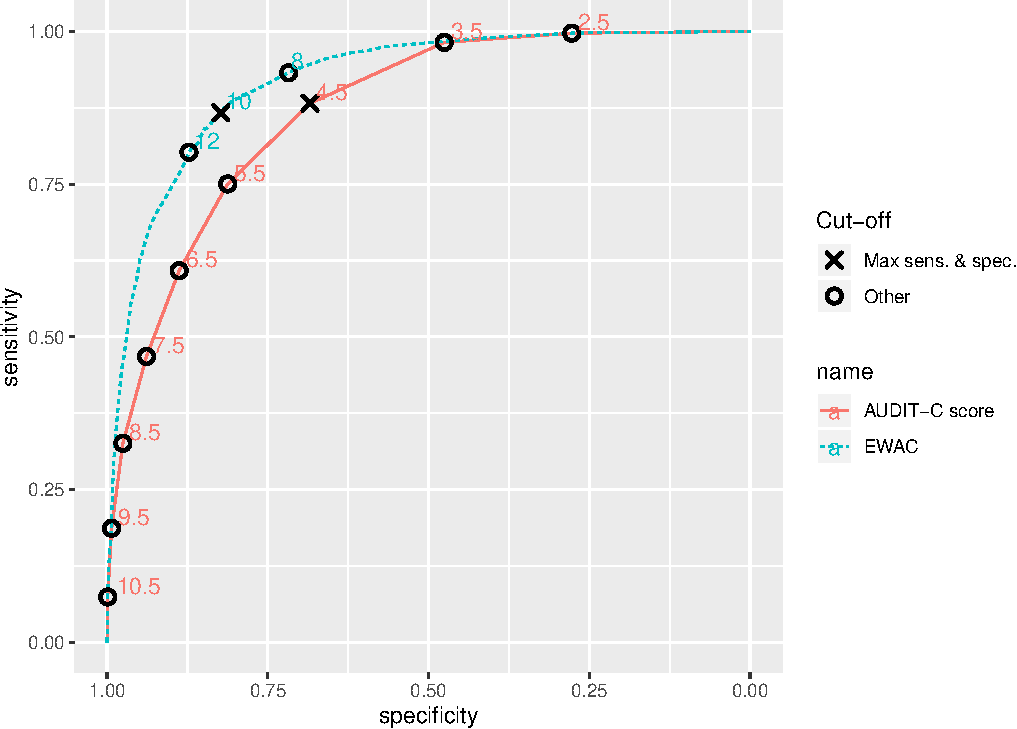
\includegraphics{analysis_files/figure-latex/unnamed-chunk-5-1.pdf}

\hypertarget{appendix-hospital-study}{%
\section{Appendix hospital study}\label{appendix-hospital-study}}

Sample size was set to power three statistical hypotheses listed in
\citep{Dutey2018}. An internal pilot conducted on 130 participants was
used to obtain estimates of the variance in MD. The study was powered to
detect a minimum MD between EWAC and TLFB of 1 unit. Using a two-sided
paired \emph{t}-test, 80\% power and 95\% confidence, the required
sample size was 387 in total. In addition, the study was powered to
detect a minimum RMSD greater than \(\text{RMSD}_{H_0} = 2\) units using
a one-sided, one-sample \(\chi^2\) test of variance. This involves
testing the null hypothesis, \(H_0: \text{RMSD}^2 = 4\) versus the
one-sided alternative hypothesis \(H_a: \text{RMSD}^2 > 4\). Dixon \&
Massey \citep{Dixon1983} set the minimum detectable value of the
variance as
\(\text{RMSD}_{H_a}^2 = \text{RMSD}_{H_0}^2 . \chi^2_{n-1, 1-\alpha} / \chi^2_{n-1, 1-\beta}\).
With \(n = 130\), \(\alpha = 0.05\) and \(\beta=.2\),
\(\text{RMSD}_{H_a} = 2.37\). The test statistic
\(\chi^2 = (n-1)\text{RMSD}^2 / 4\) follows a \(\chi^2\) distribution
with \(n-1\) degrees of freedom. The normal approximation proposed by
Dixon \& Massey \citep{Dixon1983} to the sample size require is
\[n = 1/2 \left( \dfrac{z_{1-\alpha}-z_\beta}{\ln(\text{RMSD}_{H_a}) - \ln(\text{RMSD}_{H_0})}\right)^2  \]

In our pilot study, the required sample size was 106, that is inferior
to the target pilot sample size.

\hypertarget{tables}{%
\section{Tables}\label{tables}}

Table 1: Overview of alcohol schedule used in this paper.

Survey module

Schedule

ATS QF module

On how many days, if any, did you personally drink a drink containing
alcohol in the last four weeks?

What was the maximum number of units you personally consumed on any one
day when drinking an alcoholic drink or drinks in the last four weeks?

On how many days, if any, in the last four weeks did you personally
drink\ldots{} {[}prompting in turn `51-60 units?', `41-50 units?',
\ldots{}, '1-2 units?

Health Survey for England

Thinking now about all kinds of drinks, how often have you had an
alcoholic drink of any kind during the last 12 months? {[}8 items from
`Almost every day' to `Not at all in the last 12 months'{]}

Did you have an alcoholic drink in the seven days ending yesterday?

On how many days out of the last seven did you have an alcoholic drink?

Which day last week did you last have an alcoholic drink/have the most
to drink?

Thinking about last {[}answer to previous question{]}, what types of
drink did you have that day? {[}list of 8 types of alcohol beverages{]}

{[}running through each type of beverage and recording number of units
drunk{]}

\renewcommand\refname{References}
\bibliography{bibliography}

\end{document}
